\documentclass[a4paper, twoside, 12pt]{report}

%----------------------------------------------------------------------------------------
%	Packages
%----------------------------------------------------------------------------------------

\usepackage[french]{babel}
\usepackage[utf8x]{inputenc}
\usepackage{titlesec, blindtext, color}
\usepackage[T1]{fontenc}
\usepackage{minted}
\usepackage{lscape}
\usepackage{subfigure}
\usepackage{amsmath}
\usepackage{graphicx}

\usepackage[colorinlistoftodos]{todonotes}
% make links clickable
\usepackage[hidelinks]{hyperref}

% for the table
\usepackage{multirow}
\usepackage{array}


% Sets page size and margins
\usepackage[a4paper,top=4cm,bottom=2cm,left=2cm,
	right=2cm,marginparwidth=1.75cm,headheight=2cm]{geometry}

% for the bar with date on top of each page
\usepackage{fancyhdr}

%----------------------------------------------------------------------------------------
%	Variables
%----------------------------------------------------------------------------------------

\newcommand\projectName{Projet de gestion des licences}
\newcommand\typeOfDoc{Cahier de recette}
\newcommand\titleOfDoc{\typeOfDoc \\ \hfill \\ \projectName}

\newcommand\authors{
    Sami Babigeon\\			
    Louka Boivin\\
    Kaci Hammoudi\\
    Alexis Osmont
}

\newcommand\client{M. Ziadi Djelloul}

%----------------------------------------------------------------------------------------
%	Packages configuration
%----------------------------------------------------------------------------------------

% Fancyhdr

% Redefine length
\renewcommand{\headrulewidth}{0.5pt}
\newlength{\oddmarginwidth}
\setlength{\oddmarginwidth}{0.25in+\hoffset+\oddsidemargin}
\newlength{\evenmarginwidth}
\setlength{\evenmarginwidth}{\evensidemargin+0.25in}

% Redefine the plain page style
\fancypagestyle{plain}{%
  \fancyhf{}% Clear header and footer
	\lhead{\textbf{Master SSI - Conduite de projet} \\ \projectName \\ \typeOfDoc}
	\rhead{
\includegraphics[width=3.5cm]{title/logo.png}}
	\fancyfoot[C]{\thepage}
	% Set the head width to be almost the full page width
	\fancyhfoffset[LO,RE]{\oddmarginwidth}
	\fancyhfoffset[LE,RO]{\evenmarginwidth}
}

\pagestyle{plain}

% Chapter
\definecolor{gray75}{gray}{0.75}
\newcommand{\hsp}{\hspace{20pt}}
\titleformat{\chapter}[hang]{\Huge\bfseries}{\thechapter\hsp\textcolor{gray75}{|}\hsp}{0pt}{\Huge\bfseries}

%----------------------------------------------------------------------------------------
%	Start of document
%----------------------------------------------------------------------------------------

\title{\titleOfDoc}
\author{\authors}

\begin{document}
\begin{titlepage}

\thispagestyle{empty}
\setcounter{page}{0}
\newcommand{\HRule}{\rule{\linewidth}{0.5mm}} % Defines a new command for the horizontal lines, change thickness here

%----------------------------------------------------------------------------------------
%	Logo
%----------------------------------------------------------------------------------------


\includegraphics[width=8cm]{title/logo.png}\\[1cm] % Include a department/university logo - this will require the graphicx package
 
%----------------------------------------------------------------------------------------

\center % Center everything on the page

%----------------------------------------------------------------------------------------
%	Header
%----------------------------------------------------------------------------------------

%\quad\\[1.5cm]
\textsc{\Large Université de Rouen}\\[0.5cm] % Major heading such as course name
\textsc{\large Département Informatique - Master Sécurité des Systèmes d'Informations}\\[0.5cm] % Minor heading such as course title

%----------------------------------------------------------------------------------------
%	Title
%----------------------------------------------------------------------------------------
\makeatletter
\HRule \\[0.4cm]
{ \huge \bfseries \@title}\\[0.4cm] % Title of your document
\HRule \\[1.5cm]
 
%----------------------------------------------------------------------------------------
%	Authors
%----------------------------------------------------------------------------------------

\begin{minipage}{0.4\textwidth}
\begin{flushleft} \large
\emph{Auteurs:}\\
\@author % Your name
\end{flushleft}
\end{minipage}
~
\begin{minipage}{0.4\textwidth}
\begin{flushright} \large
\emph{Client:} \\
\client % 
\end{flushright}
\end{minipage}\\[6cm]
\makeatother

%----------------------------------------------------------------------------------------
%	Date
%----------------------------------------------------------------------------------------

%{\large lorem ipsum dolor sit amet}\\[0.5cm]
%{\large \emph{lorem ipsum dolor sit amet}}\\[0.5cm]
{\large \today}\\[2cm] % Date, change the \today to a set date if you want to be precise

\vfill % Fill the rest of the page with whitespace

\end{titlepage}


% Revision Table
\chapter*{Revision}
\begin{table}[!ht] % <-- Super important in order to anchor at the top of the document
	\begin{tabular}{ | m{3cm} | m{3cm}| m{8cm} | } 
		\hline
		\textbf{Version} & \textbf{Date} & \textbf{Commentaires} \\
		\hline
			0.1 & 14/12/2021 & Création du document \\
		\hline
            0.2 & 16/12/2021 & Ajout des procédures de tests \\
        \hline
	\end{tabular}
\end{table}

\tableofcontents
\newpage

\chapter{Terminologies}

\begin{itemize}
	\item Le client est le commanditaire du projet.
	\item Un utilisateur est une personne souhaitant utiliser un logiciel du client. 
	\item Une licence est un droit accordé pour une machine et un utilisateur d'utiliser un logiciel donné.
\end{itemize}

\chapter{Contexte du projet}

Ce projet s’intitulant “Gestion et protection de licence” est proposé par notre client \\Mr.
Ziadi.\\\newline Il a pour but de créer une ou plusieur application de gestion, génération et protection 
de licence, plus particuliairement un gestionnaire de licence pour les logiciels créés par monsieur Ziadi.
\\ \newline Dans notre cas ce projet a pour but de nous apporter des connaissances et de l'experience dans les domaines traités
 mais aussi de valider notre 1 ère année de Master Informatique en Sécurité des Systèmes d’Information (SSI).\\ \newline
Nous pouvons être amenés à travailler avec Mr. Macadré pour tout ce qui est
serveur et gestion de machine virtuelles (pour leurs mise en place).\\ Nous
nous appuyons sur la Spécification Technique de Besoin, le Document d'Architecture
Logicielle, le Cahier de Recette, l’Analyse des Risques, et sur ce Plan de Développement
pour conduire le projet.

\chapter{Méthodologie de développement}

Depuis le début du projet nous travaillons selon un fonctionnement agile, avec des
réunions et des livrables réguliers, avec le client. Ce fonctionnement permet de produire de
la valeur rapidement.\\ \newline
Nous avons choisi de commencer le développement de l’application par les vues car
nous sommes partis du principe que le but final de ce projet était de rendre une application,
avec des rendus tout au long du semestre. Commencer par les vues nous permettra d’avoir
un visuel le plus rapidement possible, et d’obtenir un prototype manipulable, pour l’ensemble
des livrables.\\ \newline
Ces prototypes ne contiendront bien sûr pas l’ensemble des fonctionnalités finales
attendues par le client, mais nous permettront de réagir plus rapidement sur l’ajout de
fonctionnalités dans l’application, en fonction des demandes de ce dernier, mais nous
permettra également de faire les tests plus simplement en nous assurant que
les vues sont correctement implémentées.\\ \newline
Après avoir implémenter les vues qui permettent de naviguer entre elles, nous
commencerons par implémenter le modèle de protection et de gestion des licences.\\ \newline

La sécurité etant au coeur de notre projet, les element tel que l'obfuscation, l'injection de code et la partie 
gestion et securisation de base de données seront des element pouvouvant être gérés en divisant nos ressources
car ils sont facilement implémentable aux projet final.

\chapter{Organisation et responsabilités}

Pour organiser ce projet et travailler efficacement, nous avons affecté un rôle à
chacun. Néanmoins, tous les acteurs de ce projet auront les rôles de développeur et de
rédacteur. Voici notre organigramme :\\ \newline


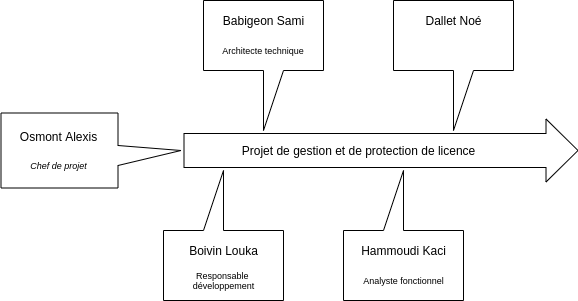
\includegraphics[width=15cm]{schema_role_projet.png}
\\ \newline
\begin{itemize}
	\item  \textbf{Chef de projet :} \newline
	\begin{itemize}
		\item Organiser et conduire le projet de bout en bout.
		\item Décide des actions et résout les désaccords entre les membres du projet.\newline
	\end{itemize}
	\item \textbf{Architecte tehcnique :} \newline
	\begin{itemize}
		\item Garantit l'encadrement et la maintenance technique du projet.
		\item Assure la fiabilité, la performance et l'évolution du système d'information.\newline
	\end{itemize}
	\newpage
	\item \textbf{Analyste fonctionnel :} \newline
	\begin{itemize}
		\item Schématise l’interface de l’application.
		\item Se charge de la conception générale de l’interface, de la clarté de la
		navigation, de l’optimisation des parcours ainsi que de la qualité des
		contenus.\newline
	\end{itemize}
	
	\item \textbf{Responsable développement :} \newline
	\begin{itemize}
		\item Définit les besoins du client.
		\item Assure le suivi fonctionnel.\newline
	\end{itemize}
	
	
\end{itemize}

\chapter{Organigramme des tâches}
L'organigramme des tâches present ci-dessous n'est qu'une capture du momment. En effet celui-ci sera mis à jour en fonction 
des possibles nouvelles tâches qui viendront le completer. \\

L'organigramme est disponible en annexe pour une meilleur lisibilité.\\ \newline
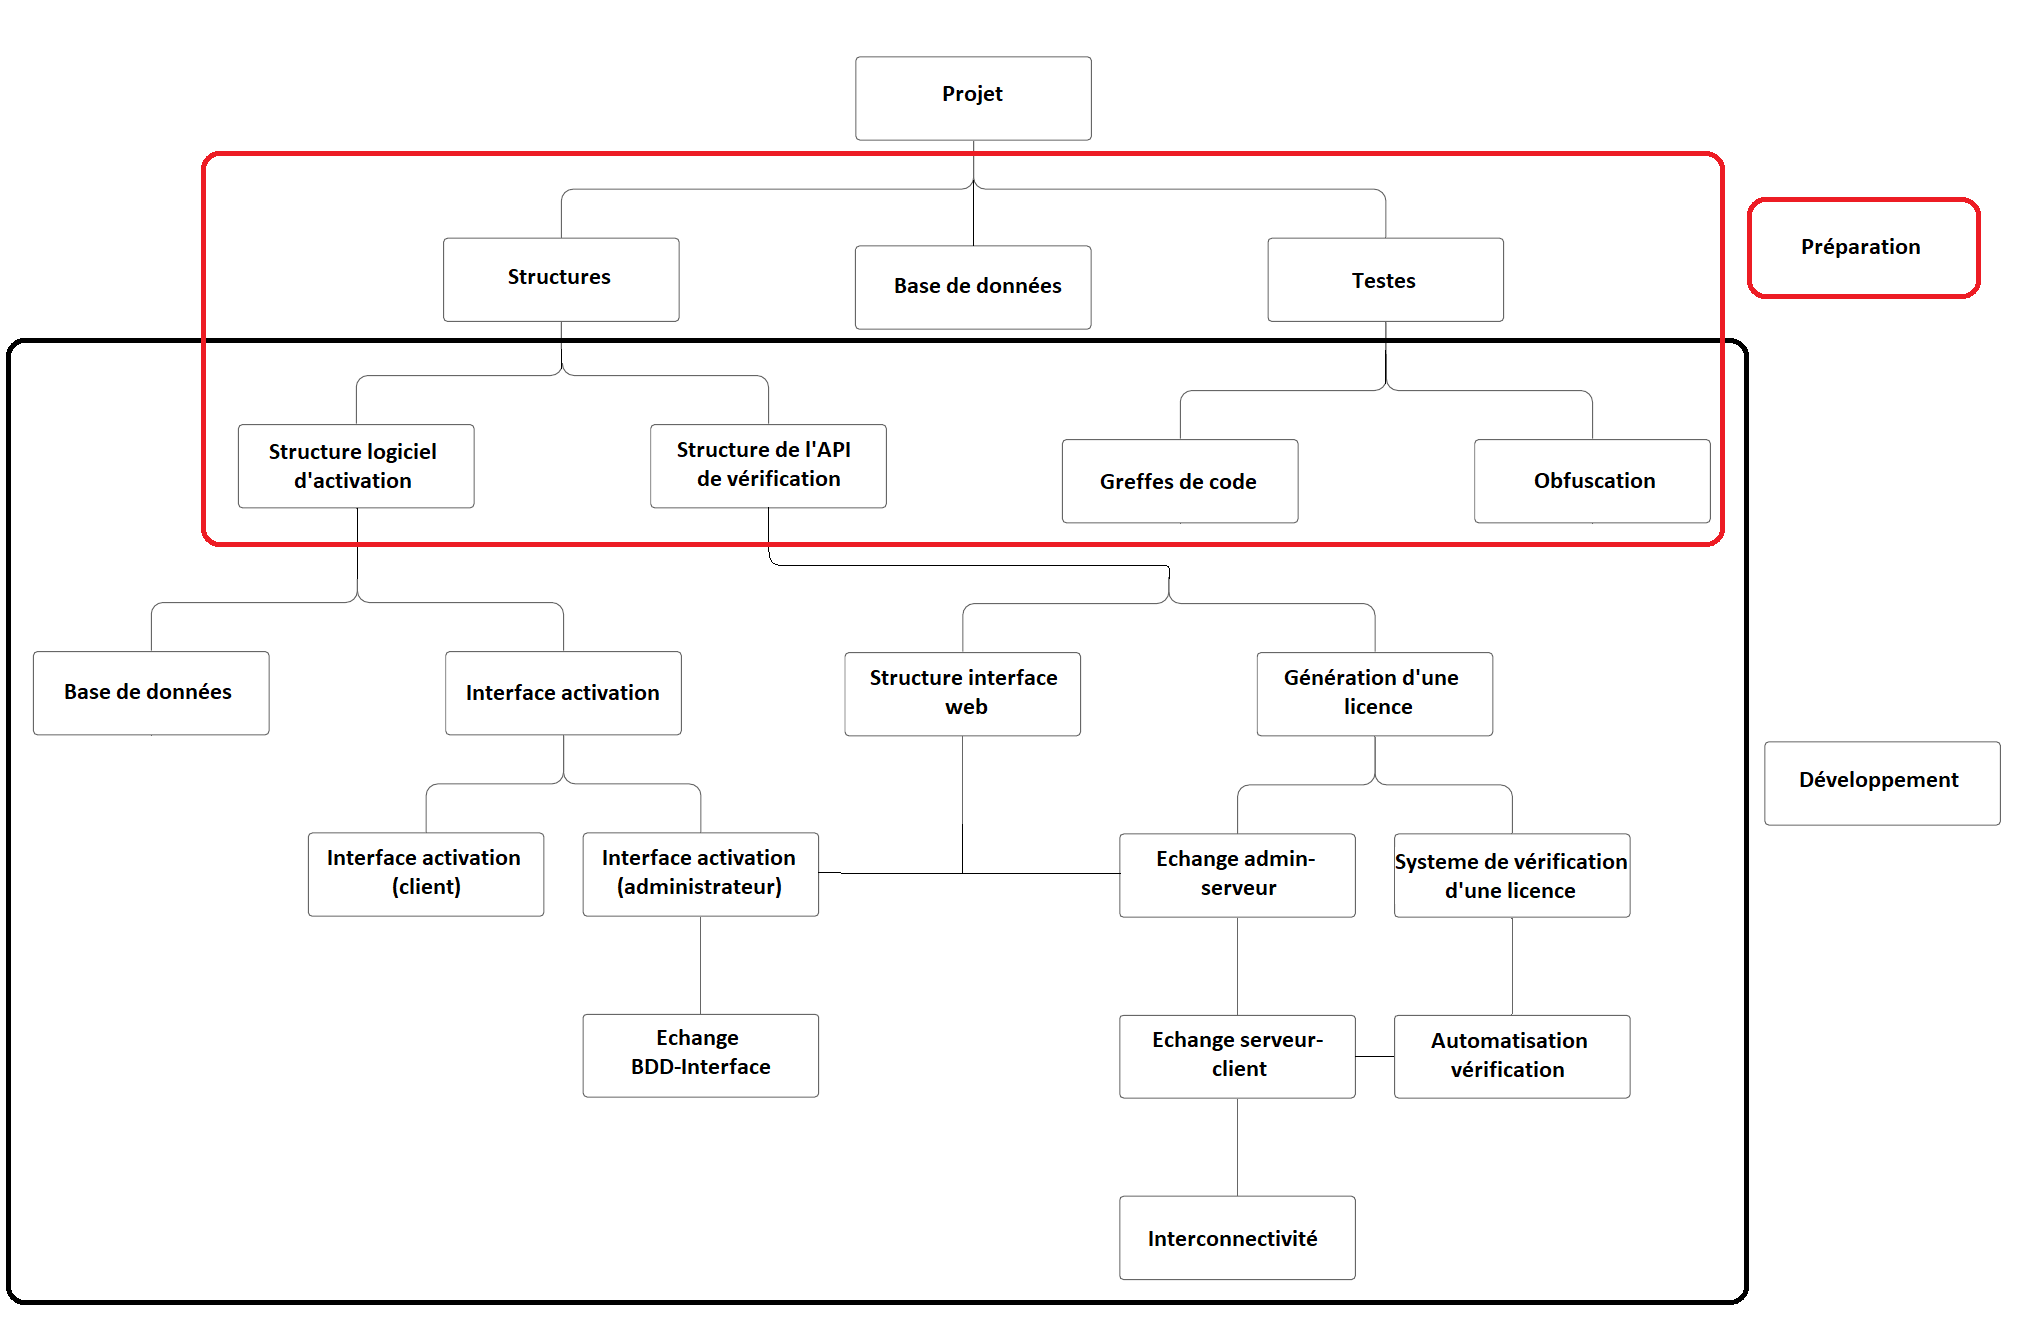
\includegraphics[width=18cm]{organi.png}

\chapter{Evaluation du projet et dimensionnement des moyens}
\section{Charge et répartition par phase}
Nous avons divisé la charge et la répartition par phase. La premiere phase est intitulé «Préparation». Cette premiere phase permet
de donner un temps aproximatif de structuration du projet, de verification des répartition des tâches et des phase de test qui permettront des évaluations de temps de
développement plus précises tel que les testes de greffe de code ou ceux d'obfucation. Cette phase d'après nos estimations nécessiterait 4 semaines, 2 semaines de 
répartition et de teste puis deux semaine de strucutre de projet qui se terminerait par une réunion avec le client pour attester de l'evaluation du temps
et des ressources nécessaires au bon déroulement du projet.
\\ \newline

La seconde phase est celle du developpement qui nécessitera le plus de temps.En effet nous avons évalué cette phase à deux mois de travail.
Cette phase se decompeserait en 3 parties : \newline

\begin{itemize}
	\item Phase post-préparation : 2 semaines\\ 
	Cette phase et nécessaire pour structurer le projet et les parties de developpement avant la séparation des tâches principale, En effet apres la phase de préparation 
	il nous faut créer une structure de projet pour que chaque personne puisse travailler sur des bases solide sans gener l'avancement sur les partes des 
	autres membres du projet. \newline
	\item Phase de développement : 4 semaines\\
	La phase de développement est quant à elle la principale, elle consiste à repondre aux besoins de chaque element du projet. Cette phase permet 
	à tous les differents élément d'être fonctionnel.
	\item Phase d'interaction : 3 semaines\\
	La derniere phase consiste à connecter tous ces développements, le coeur de cette partie sera donc de connecter les elements entre eux. (serveur -> adiminstrateur; téléchargement du logiciel d'activation -> client; ....)
\end{itemize}
\newpage
\section{Besoin en moyen et en ressources}
Nécessaire au développement et testes:
\begin{itemize}
	\item Serveur
	\item Base de données
	\item Logiciels du client
	\item Dépot(s) Git \\ \newline
\end{itemize}
après une concertation entre les membres du projet et leurs connaissances personnelles, l'estimation de temps fait est de
  110 heures en moyenne de travail afin de remplire les exigences du client, nos exigences personnelles et de terminer les tâches definis
	dans l'organigramme ci-dessus.\\ \newline

	Remarque : Le chapitre ci-dessus «Evaluation du projet et dimensionnement des moyens» est à titre indiquatif, en effet ce chapite comme le chapitre précédent 
	n'est qu'une évaluation. Ils seront donc amenés à changer au cours du développement du projet.

\chapter{Planning général}
Le diagramme de gantt present ci-dessous n'est qu'une capture du momment. En effet celui-ci sera mis à jour en fonction de l'avancement
du projet, de la répartition des tâches et des possibles nouvelles tâches qui viendront le completer. \\

Le diagramme de Gantt est disponible en annexe.\\ \newline
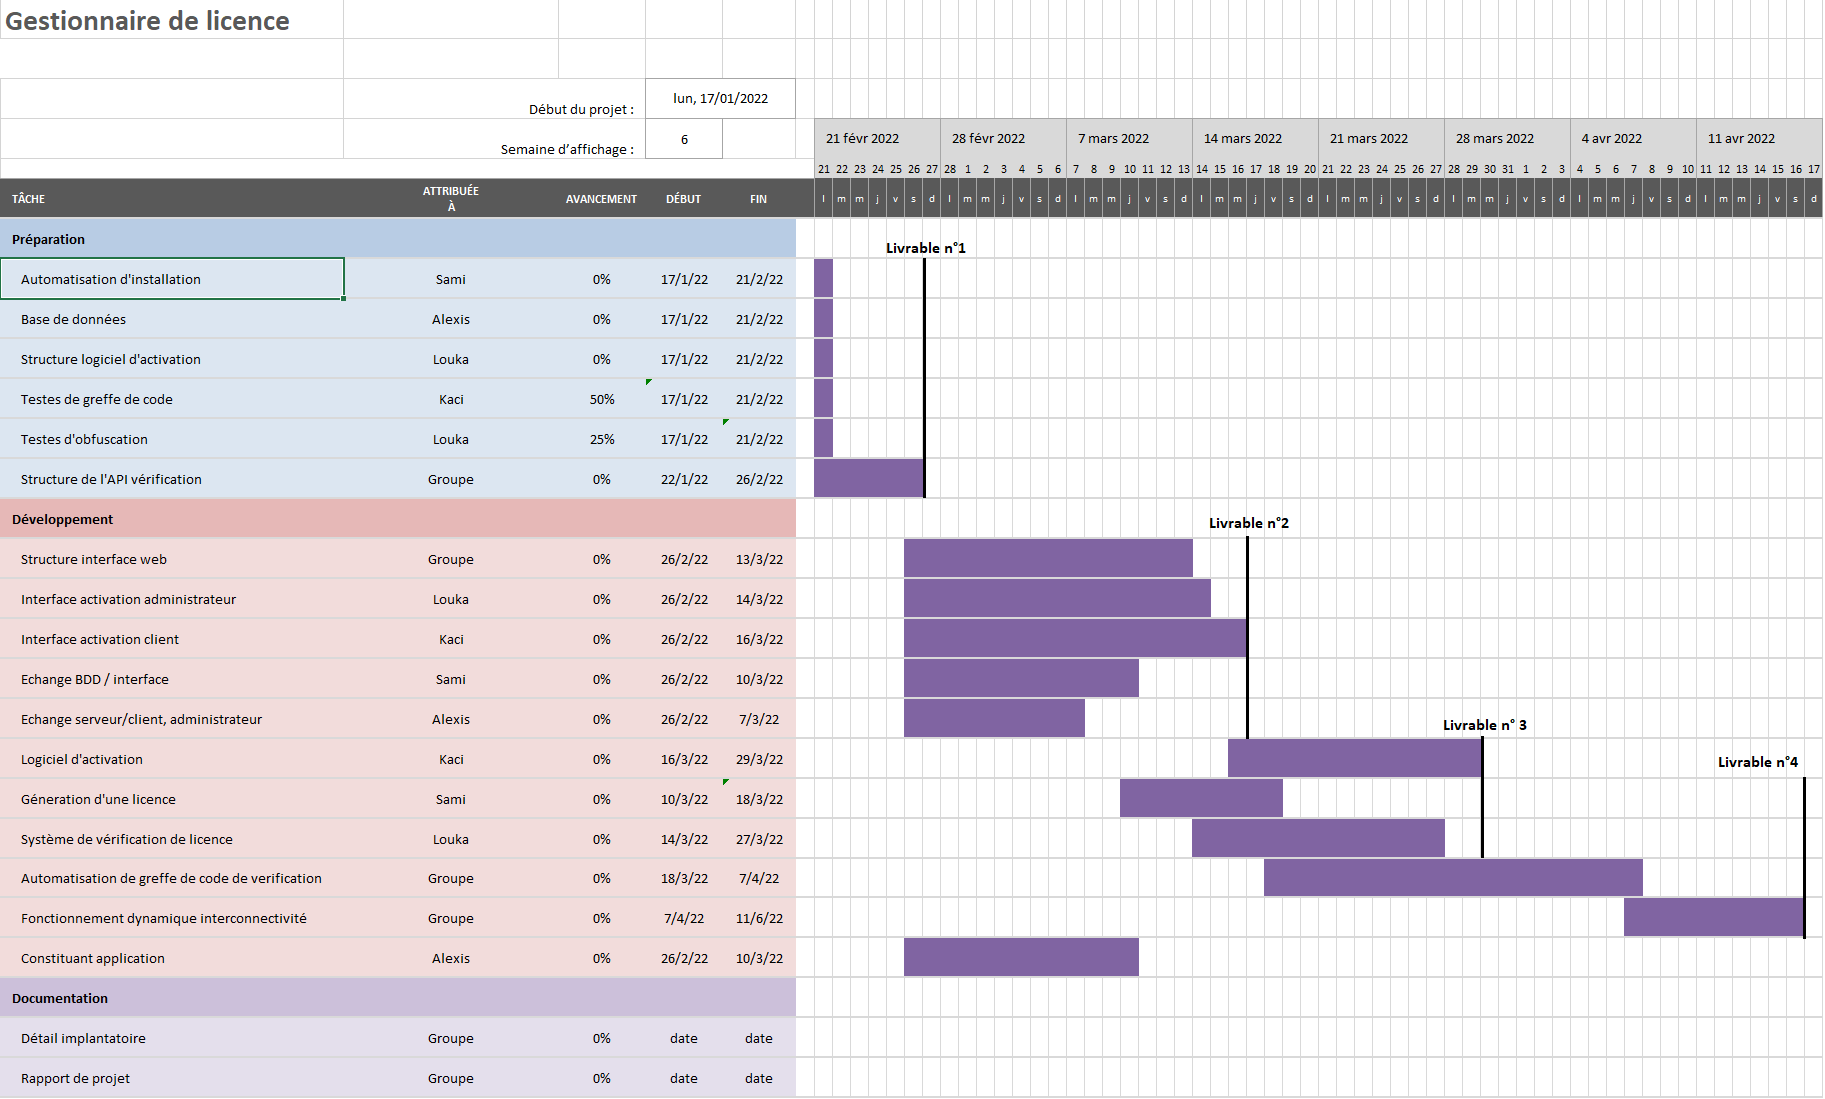
\includegraphics[width=17cm]{Gantt.png}

\chapter{Procédés de gestion}
\section{Gestion de la documentation}
		Au second semestre, nous devrons fournir les documents suivants :
		\begin{itemize}
			\item Documentation technique : décrit le fonctionnement détaillé de l’application.
			\item Notice d’utilisation : support explicatif du maniement de l’application.
			\item Des comptes rendu post-réunion après chaque réunions.
			\item Des livrables pré-réunion chaque deux semaine.\\ \newline
		\end{itemize}
	
		\section{Gestion des configurations}
		Lors du développement, nous utiliserons le GitLab fourni par l’université ainsi que Github. Chacun
		aura une tache de développement et il y aura des réunions de travail en groupe qui donneront les versions
		stable du code (pré-réunion) et des documentations (en Latex). Chacun aura son espace pour
		permettre à tous de fusionner sa partie à la branche principale.



\chapter{Revues et points clefs}

L'objectif dans notre cas est de faire suivre notre projet par note client,
nous fournirons donc au client un livrable toutes les deux semaines, et nous effectuerons
quelques jours après chaque livraison une réunion avec lui pour voir les modifications à
apportées. Des dates prévisionnelles ont été indiquées dans le diagramme de Gantt.\\

Comme précisé dans la partie «Evaluation du projet et dimensionnement des moyens» une réunion sera organisée à chaque fin de phase pour faire 
une revues des points clefs du projet et pour informer le client de l'avancement du projet et de ses besoins.

\chapter{Procédure de suivi d'avancement}

Pour avancer rapidement et efficacement tout en évitant les hors-sujet, nous avons
décidé d’utiliser diverses plateformes pour suivre l’avancement de chacun, et de ce fait,
d’éviter qu’un membre ne soit en attente. Les plateformes utilisées sont les suivantes :\\ \newline

\begin{itemize}
	\item Discord :\\
	Cet outil nous permet de communiquer rapidement entre nous et
de faire des audios / visioconférences pour nos réunions. Il est aussi très utile
pour communiquer rapidement et faire des annonces importantes (réunions,
vérification d’un mail avant son envoi, etc.) et pour partager / archiver les
comptes rendus de toutes les réunions.\\
	\item Trello :\\
	Cet outil nous permet de répartir et de savoir sur quelle tâche
travaillent les membres de l’équipe et de connaître leur avancement.\\
	\item GitHub :\\
	L’université nous a fourni cet outil qui est très pratique pour stocker
les documentations produites et le code source de l’application que nous
aurons à faire lors de la phase de développement.\\
	\item Google docs / GitHub :\\
	Ces outils nous permettent de réaliser les documents demandés
pour la matière Gestion de Projet. Google Docs nous permet de travailler à
plusieurs sur un même document. Les modifications apparaissent en temps
réel et sont sauvegardées sur une période de trente jours. Il est donc possible
de consulter des versions antérieures de nos documents en quelques clics.\\
	\item Réunions :\\
	Le meilleur moyen de travailler efficacement reste le fait d'organiser des réunions en physique 
	plutot que des appels ou des echanges de messages. C'est pourquoi nous organisons régulièrement des réunions
	entre membre du projet pour faire un point définir les objectif et avancer sur le projet. \newline

Pour tenir de l'avancement du projet nous planifions des seances de travails et des réunions hebdomadaire pour traiter
aussi bien de l'aspect technique que de l'aspect gestion de projet. Des comptes rendu de réunion sont effectués après chaqu'une d'entre elles.
\end{itemize}


%\bibliographystyle{unsrt}
%\bibliography{bibs/sample}
%\addcontentsline{toc}{chapter}{Bibliographie}

\end{document}
